%%% ---------------------------------------------------------------------------------
%%% Vorlage Abschlussarbeit (LaTeX)
%%% 
%%% V1   03/2017, Stefan Etschberger (HSA)
%%% V1.1 04/2021, rnw-hack für biblatex-run
%%% V2   05/2021, Titelblatt und Erweiterungen: Stefan Jansen (HSA)
%%% V2.1 05/2021, Trennung von R-Support und einfachem LaTeX: Phillip Heidegger (HSA)
%%% V2.2 01/2024, Anpassung an THA-Layout
%%% V3   01/2024, I18n
%%% V3.1 10/2024, Phillip Heideger, Online Version präferiert, Reparatur langes Inhaltsverzeichnis,
%%%               Erklärung Referenzen, blau für Refs & Links
%%% ---------------------------------------------------------------------------------
\documentclass[12pt,a4paper%
              ,oneside     % fuer PDF-Abgabe, bei Druck twoside
              ,titlepage
              ,DIV=13
              ,headinclude
              ,footinclude=false%
              ,cleardoublepage=empty%
              ,parskip=half,
              BCOR=0mm,
              ]{scrreprt}

\usepackage[utf8]{inputenc}
\usepackage[T1]{fontenc}

\usepackage[authorName={Jonas Kraus}
           ,authorEnrolmentNo={30041777}
           ,authorStreet={Afrastraße 40}
           ,authorZip={86316}
           ,authorCity={Friedberg}
           ,authorEMail={jonas.kraus@tha.de}
           ,authorSignaturePlace={Augsburg}
           ,studyProgram={Informatik}
           ,thesisType={Bachelorarbeit}
           ,thesisTitle={Visualisierung von Montageregeln für Rauchmelder mithilfe von Augmented Reality}
           ,studyDegree={{Bachelor of Science (B.\,Sc.)}}
           ,faculty={{Fakultät für \\ Informatik}}
           ,topicAssignment={\today}
           ,submissionDate={\today}
           ,defenseDate={\today}
           ,nonDisclosure={false}
           ,supervisor={Prof.~Dr.~Michael Strohmeier}
           ,supervisorDeputy={Prof.~Dr.~Michael Strohmeier}
           ,language={de}
           ]{THA-Abschlussarbeit}

% ====== mögliches Setup fürs PDFs =======
\hypersetup{
  colorlinks=true,
  allcolors = THAi-Blue, % oder THAred ??
  linktocpage  
}
% Siehe:
% https://ctan.net/macros/latex/contrib/hyperref/doc/hyperref-doc.pdf
% S. Kap. 5, S. 10 ff

% Ohne diese Zeile: Mit klickbaren links
% \hypersetup{draft}


% Literaturdatenbank (.bib-Datei) aus Citavi o.ä.
\bibliography{Literatur_Abschlussarbeit}

\graphicspath{{Bilder/}}

\usepackage{caption}
\DeclareCaptionLabelFormat{something}{#2.#1.}
\captionsetup[lstlisting]{labelformat=something}

\begin{document}

% Sprachauswahl zum Umschalten innerhalb des Textes. 
% Alternativen: \thesisLanguage, ngerman, english
\selectlanguage{\thesisLanguage}

\pagenumbering{roman}
\setcounter{page}{1}

\THAtitlepage

\tableofcontents

%%% --------------------------------------------------
%%% Ab hier: Inhalt
%%% --------------------------------------------------

\setcounter{page}{1}
\pagenumbering{arabic}

\chapter{Hier beginnt das erste Kapitel}

% -----------------------------------------------------
\section{Wie verweist man auf Quellen?}

Hier wird \citet{Neumann:1977} zitiert. Zitate sollten in den Text eingebunden werden, zum Beispiel eine Quelle aus einem Tagungsband, hier von \citet{Bauer} oder ein Artikel aus einer Fachzeitschrift (auf den dann in einer Klammer beispielsweise bei \cite{Fox:2002} verwiesen wird). 

Noch ein Absatz mit einem Zitat aus einem Buch, nämlich von \citet{R:Chambers:1998}. Webseiten, zum Beispiel das Dokument von \citet{xmlComparingSchemata} sollten nur äußerst sparsam referenziert werden. 

Hier wird ein Buch zitiert, nämlich das von \citet{darwin}. Die Arbeit von \citet{meulman} ist in einer wissenschaftlichen Fachzeitschrift veröffentlicht worden. Ein Beispiel für einen Aufsatz in einem Tagungsband liefert \citet{banzhaf96effect}. In Ausnahmefällen zu zitieren ist eine unveröffentlichte Abschlussarbeit, zum Beispiel eine Diplom-, Bachelor-, oder Masterthesis, wie die von \citet{holzheuer}. Ganz selten ist man gezwungen Manuale oder Referenzen zu referenzieren, die nur im Internet zugänglich sind und zudem keinen ausgewiesenen Autor haben wie zum Beispiel die Anleitung vom \citet{hornik} oder der Aufsatz von \citet{xmlComparingSchemata}.

% -----------------------------------------------------
\section{Einbinden von Grafiken}

Es folgt die Abbildung~\ref{fig:Gauss} auf Seite \pageref{fig:Gauss}, die dynamisch (gleitend) eingebunden wird. Das ist typischerweise eine gute Idee und man sollte Grafiken, wenn es nicht unbedingt anders gemacht werden soll von LaTeX automatisch positionieren lassen.

\blindtext 

\begin{figure}
\centering
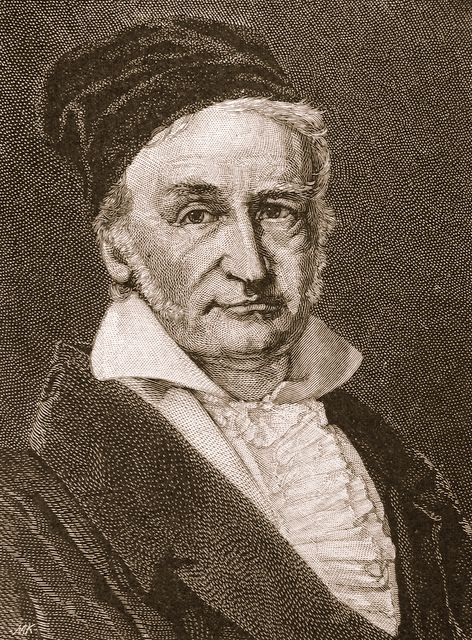
\includegraphics[ angle=0, width=.3\textwidth]{karl_friedrich_gauss}
\caption{\index{Grafik}\index{jpg}Ein jpeg-Bild, hier mit Gauß darauf\label{fig:Gauss}}\par
\end{figure}

\blindtext \blindtext 

\blindtext



% -----------------------------------------------------
\section{Einträge im Stichwortverzeichnis}

Einträge im Stichwortverzeichnis können über den \lstI{index}-Befehl generiert werden. Zum Beispiel soll der Begriff \emph{Bachelorarbeit}\index{Bachelorarbeit} hier referenziert werden. Außerdem sollen noch die Begriffe Apfel\index{Apfel}, Birne\index{Birne} und Zebra\index{Zebra} ins Verzeichnis. Damit unter dem Buchstaben mehr als ein Eintrag steht, nehmen wir noch \emph{Buch}\index{Buch} und Brille\index{Brille} auf. 

\section{Dynamische Tabellen aus beliebigen Quellen}

In dieser Version kein Support für R-Code. 

\blindtext 

\blindtext \blindtext

\blindtext

\blindtext

\section{Grafiken aus R}

In dieser Version kein Support für R-Code. Die Grafiken können
natürlich durch das Makefile passend generiert werden, und dann
auch eingebunden werden.

\blindtext

\blindtext

\blindtext \blindtext \blindtext


%\lstset{
    %language=[LaTeX]TeX,
    %backgroundcolor = \color{black!10},
    %basicstyle=\ttfamily\normalsize\color{black},
    %breaklines=true,
    %columns = fullflexible, 
    %framexleftmargin = 3pt,
    %frame = single,
    %identifierstyle=\ttfamily\color{black},
    %keywordstyle=\ttfamily\color{black},
    %otherkeywords = {usetheme, useinnertheme, useoutertheme,usefonttheme, usecolortheme},
%}


\chapter{Noch ein paar Textbestandteile}
 
 \section{Mathematiknotation}

Hier kommt eine abgesetzte Formel ohne Nummerierung:
%
\begin{align*}
\frac{a+1}{b+1} \quad \tfrac{a+1}{b+1} \quad  \dfrac{a+1}{b+1} \quad \nicefrac{a}{b}
\end{align*}
%
In einem Text ist $\nicefrac{1}{8}$ schöner als $\frac{1}{8}$. 
%	
\begin{align}
\label{eq:pythagoras} a^2 + b^2  & = c^2 \\ 
\label{eq:fermat} a^n + b^n & = c^n \\ 
\label{eq:schoen} \textsf{e}^{\textsf{i}\pi} +1 & = 0 \quad \text{mit} \quad  \textsf{i}^2  = -1   
\end{align}	
%
\begin{align}
f(x) = A \sin(\alpha x + b) + \log(x) \cdot \sin\left(\frac{x}{y}\right) \\
g(x) = \left(\frac{\ \ x (1-x^2)\ \ }{\frac{1}{2-x^2 +3x -y^2}} \right)
\end{align}
%	
Man nennt die %Bsp. um auch "Formel" klickbar und farbig zu machen:
  \hyperref[eq:pythagoras]{Formel~\eqref{eq:pythagoras}}
  % es geht auch, dies erfordert eine Anpassung in der STY Datei um cleverref zu laden (oder laden des Packets im Header):
  % cref kann dann Referenzen basierend auf dem Counter automatisch korrekt generieren, d.h. "Kapitel X, Abschnitt Y, Tabelle 2, Gleichung (7), etc."
  % \cref{eq:pythagoras}
  % Formel~\eqref{eq:pythagoras}
den Satz des Pythagoras. Die Fermat'sche Vermutung besagt, dass Gleichung~\eqref{eq:fermat} keine positiven ganzzahligen Lösungen $a, b, c$ für $n \ge 3$ hat und wurde 1994 von Andrew Wiles und Richard Taylor bewiesen. 

Gleichung~\eqref{eq:schoen} wird oft als die schönste Gleichung der Mathematik bezeichnet. Um Konstanten von Variablen zu unterscheiden sollte man die Eulersche Zahl sowie die imaginäre Einheit in Formeln aufrecht setzen. Das geht mithilfe von \newline \lstinline!\text{<zeichen>}!. 
%
\begin{align}
\label{eq:binomial}
(a+b)^n = \sum_{k = 0}^{n} \binom{n}{k} a^k b^{n-k}
\end{align}	
%	
Der junge Carl-Friedrich Gauss fand zu Schulzeiten die Formel $\sum_{j = 1}^N = \frac{1}{2}N(N+1)$. Innerhalb von Text ist es auch möglich die Grenzen ober- und unterhalb zu setzen. Dafür existiert der Befehl {\lstI{limits}}. Das sieht dann so aus: $\zeta(x) = \sum\limits_{n=1}^{\infty} \frac{1}{n^x}$, und erhöht dann etwas unglücklich den Zeilenabstand. Ein paar gesetzte Formeln: % mit den neu definierten Befehlen:	
%
\begin{align*}
\sin(x)^2 + \cos(x)^2 & = 1 &
\int_{1}^{\infty} \frac{1}{x^2} \, \textrm{d}x & = 1 \\
\frac{\partial f(x, y)}{\partial y} & = x^2 + 2y
\end{align*}
%
Diese Formeln wurden hier mit der \texttt{align*}-Umgebung (mit Stern "`*"') erstellt, daher sind sie nicht nummeriert. Mit dem Kaufmanns-und (\&) kann man Gleichungen setzen: hier hat jede Zeile ein \texttt{\&} unter vor dem \texttt{=}.  $\cdot$ ist der Malpunkt, $\cdots$ und $\vdots$ sind viele Punkte, und $\ddots$ sind diagonal. Dies ist besonders bei der Darstellung von großen Matrizen sinnvoll, zum Beispiel:
%
\begin{align*}
A= (a_{ij})_{m,n} = \begin{pmatrix} a_{11} & a_{12} & \cdots & a_{1n} \\ a_{21} & a_{22} & \cdots & a_{2n} \\ \vdots  & \vdots & \ddots & \vdots \\  a_{m1} & a_{m2} & \cdots & a_{mn} \end{pmatrix} 
\end{align*}
%
\begin{align*}
\left(\frac{1}{2} + \frac{3}{5}\right) \cdot 7 = \frac{77}{10}
\end{align*}

Für logische Zusammenhänge braucht man oft die Implikation $\implies$ oder die Äquivalenz $\iff$. Die Verneinung einer Aussage kann man entweder so $\neg A$ oder auch $\overline{A}$ darstellen. Für die logischen Vernüpfungen gibt es $\wedge$ und $\vee$ (so wie jede Menge anderer Zeichen...). 

Manchmal braucht man auch die Menge der natürlichen Zahlen, dafür nimmt man das Paket \texttt{dsfont}, so dass man zum Beispiel schreiben kann:
%
\begin{align}
\mathds{N} & = \{1, 2, 3, \cdots \} \\
\mathds{Z} & = \{0, \pm 1, \pm 2, \pm 3, \cdots \}
\end{align}
%
und analog natürlich auch $\mathds{Q, R, C}$ oder bleibige andere Großbuchstaben: 
%
\begin{align*}
\mathds{A, B, D, E, F, G, H, I, J, K, L, M, O, P, S, T, V, W, X, Y}.
\end{align*}
%
Wenn man Matrizen braucht, so gibt es diverse Matrix-Umgebungen:
%
\begin{align*} 
\begin{matrix} a_{11} & a_{12} \\ a_{21} & a_{22} \end{matrix} \quad  
\begin{pmatrix} a_{11} & a_{12} \\ a_{21} & a_{22} \end{pmatrix} \quad  \begin{vmatrix} a_{11} & a_{12} \\ a_{21} & a_{22} \end{vmatrix} \quad  \begin{Vmatrix} a_{11} & a_{12} \\ a_{21} & a_{22} \end{Vmatrix} \quad  \begin{bmatrix} a_{11} & a_{12} \\ a_{21} & a_{22} \end{bmatrix} \quad  \begin{Bmatrix} a_{11} & a_{12} \\ a_{21} & a_{22} \end{Bmatrix} \quad  \end{align*}
%
Hier wurden der Reihe nach die Umgebungen \texttt{matrix}, \texttt{pmatrix}, \texttt{vmatrix}, \texttt{Vmatrix}, \texttt{bmatrix}, \texttt{Bmatrix} verwendet. Zur Fallunterscheidung gibt es die \texttt{cases}-Umgebung:
%
\begin{align*}
|x| = \begin{cases}
\phantom{-}x & \text{falls } \, x>0 \\ -x & \text{falls } x< 0
\end{cases}
\end{align*}
%
Will man unter oder über Terme etwas schreiben, so kann gibt es die Befehle {\lstinline!\underbrace{}!} und {\lstinline!\overbrace{}!}
\begin{align}
\underbrace{x^3 + 7x^2 + 3x -7 = 0}_{\text{notwendige Bedingung}}  \quad \overbrace{f'(x) = 0}^{\text{Nullstellen}}.
\end{align}	
%		
Mit {\lstinline!\underline{}!} und {\lstinline!\overline{}!} können Ausdrücke in einer Mathematikumgebung unterstrichen bzw. überstrichen (gibt es das Wort in diesem Zusammenhang?!) werden:
%
\begin{align*}
\underline{a} = \vec{a} = \frak{a} \quad \text{oder} \quad \overline{a + \text{i} b} = a - \text{i} b
\end{align*}
%
Oft sind in wissenschaftlich-mathematischen Texten griechische Buchstaben nötig:
%

\begin{minipage}{.45\textwidth}
\centering

\begin{tabular}{ccl} \toprule
Klein & Groß & Name \\ \midrule
$\alpha$ & \textrm{A} & Alpha \\    
$\beta$ & \textrm{B} & Beta \\  
$\gamma$ & $\Gamma$ & Gamma \\  
$\delta$ & $\Delta$ & Delta \\ 
$\epsilon$, $\varepsilon$ & \textrm{E} & Epsilon \\
$\zeta$ & \textrm{Z} & Zeta \\
$\eta$ & \textrm{H} & Eta  \\
$\theta$ , $\vartheta$ & $\Theta$ & Theta \\
$\iota$ & \textrm{I} & Iota \\
$\kappa$ & \textrm{K} & Kappa \\
$\lambda$ & $\Lambda$ & Lambda \\
$\mu$ & \textrm{M} & My \\ \bottomrule
\end{tabular}
\par\end{minipage}
%
\hfill
%
\begin{minipage}{.45\textwidth}
\centering
\begin{tabular}{ccl} \toprule
Klein & Groß & Name \\ \midrule
$\nu$ & \textrm{N} & Ny \\
$\xi$ & $\Xi$ & Xi \\
\textrm{o} & \textrm{O} & Omikron \\
$\pi$ & $\Pi$ & Pi \\
$\rho$, $\varrho$ & \textrm{P} & Rho \\
$\sigma$ & $\Sigma$ & Sigma  \\
$\tau$ & \textrm{T} & Tau \\
$\upsilon$ & $\Upsilon$ & Ypsilon \\
$\phi$,$\varphi$ & $\Phi$ & Phi \\
$\chi$ & \textrm{X} & Chi \\
$\psi$ & $\Psi$ & Psi \\
$\omega$ & $\Omega$ & Omega \\ \bottomrule
\end{tabular}
\par
\end{minipage}


\section{Aufzählungen}

Es gibt im wesentlichen drei Formen von Listen bzw. Aufzählungen

\subsection{Nummerierte Aufzählungen}
Bei der \texttt{enumerate}-Umgebung wird durchgezählt
 \begin{enumerate}
  \item Die erste Ebene 
   \begin{enumerate}
    \item zweite Ebene
    \item zweiter Eintrag zweite Ebene
    \item Hier nun die dritte Ebene:
      \begin{enumerate}
        \item Meistens ist es nicht nötig noch weiter zu schachteln
        \item aber sollte man es doch mal brauchen, so steht auch noch 
         \begin{enumerate}
           \item weitere 
           \item Ebenen 
           \item zur Verfügung.
         \end{enumerate}
        \item Aber meist reicht diese hier!  
      \end{enumerate}
    \end{enumerate}
  \item Zweiter Eintrag in der ersten Ebene
 \end{enumerate}

\subsection{Ohne Nummerierung}
 
Sollte man keine Nummerierung benötigen, so gibt es auch die einfachen Spiegelstriche. 
Die \texttt{itemize}-Umgebung stellt einfache Spiegelstriche oder deren Pendants zur Verfügung. 

\begin{itemize}
   \item Die erste Ebene 
   \begin{itemize}
    \item zweite Ebene
    \item zweiter Eintrag zweite Ebene
    \item Hier nun die dritte Ebene:
      \begin{itemize}
        \item Meistens ist es nicht nötig noch weiter zu schachteln
        \item aber sollte man es doch mal brauchen, so steht auch noch 
         \begin{itemize}
           \item genau eine weitere 
           \item Ebene 
           \item zur Verfügung.
         \end{itemize}
        \item Aber meist reicht die dritte schon.  
      \end{itemize}
    \end{itemize}
  \item Zweiter Eintrag in der ersten Ebene
 \end{itemize}

\subsection{Beschreibende Aufzählungen}

\begin{description}
\item[description] Diese oberste Aufzählungsebene hier ist mit Hilfe der \texttt{description}-Umgebung gemacht. Das hat den Vorteil, dass alle folgenden Zeilen eingerückt sind, was den gesamten Text leserlich macht. 
\item[Fortsetzung] Der zu beschreibende Titel der Aufzählung wird dabei in eckigen Klammern hinter das \texttt{item} gesetzt. Dies ist auch bei anderen Aufzählungen möglich.
\end{description}

Es gibt einige Pakete, die bei den Aufzählungen helfen. Das beste ist das \texttt{enumitem}-Paket, mit dem man sämtliche Parameter einer Aufzählung kontrollieren kann, seien es die Nummerierung, Abstände oder das Einrücken. 

Schön ist außerdem die Option \texttt{[resume]} wenn durchnummerierte Aufzählungen fortgeführt werden sollen
\begin{enumerate}
\item Text in einer Aufzählung
\item und noch ein Punkt
\end{enumerate}
%
Nun ein kurzer Text, der außerhalb der Aufzählung ist, damit man besser erkennen kann was passiert, wenn die Aufzählung weiter gehen soll.
%
\begin{enumerate}[resume]
\item Text in der zweiten Aufzählung mit \texttt{[resume]}-Option
\item mit dem Befehl \texttt{addtocounter} kann man auch den Counter hochzählen
\addtocounter{enumi}{4}
\item so dass hier zum Beispiel um 4 hochgezählt wurde.
\end{enumerate}

\section{Referenzen}\label{sec:referenzen}

Latex bietet viele Möglichkeiten an, innerhalb des Dokuments auf
andere Teile zu verweisen.  Sie müssen an der Überschrift, Gleichung
etc., die referenziert werden soll, ein Label anbringen. Mit dem
Befehl \verb|\ref| können Sie dann auf das Label verweisen, z.B.
Abschnitt~\ref{sec:referenzen}. Nachteilig ist hier, dass nur die
Zahl, d.h. der Counter als Link dargestellt wird, und Sie manuell
jeweils den passenden Begriff, d.h. Abschnitt, Gleichung, etc.
anbringen müssen. 

Um hier ein schöneres Ergebnis zu erzielen, gibt es viele Optionen. In
der Vorlage wird das Packet \verb|hyperref| in der Datei
\verb|THA-Abchlussarbeit.sty| geladen. Dieses Packet ermöglicht
z.B. mithilfe des Befehls \verb|hyperref| den Text sowie das Ziel
einer Referenz zu setzen.  So wird
\begin{lstlisting}
  \hyperref[sec:referenzen]{hier}
\end{lstlisting}
z.B. so dargestellt: \hyperref[sec:referenzen]{hier}.
Der generierte Link referenziert wie oben auf
Abschnitt~\ref{sec:referenzen}.

Als ersten Schritt für eine Verbesserung bieten sich somit folgendes an.
Sie können nämlich \verb|ref| und \verb|hyperref| kombinieren, so dass z.B.
\begin{lstlisting}
\hyperref[sec:referenzen]{Abschnitt~\ref{sec:referenzen}}  
\end{lstlisting}
zu folgender schönerer Ausgabe führt: 
\hyperref[sec:referenzen]{Abschnitt~\ref{sec:referenzen}}.

Allerdings bedeutet dies viel manuelle Arbeit, denn wie Sie leicht
sehen können, sind dann die Befehle deutlich länger, und auch
fehleranfällig, da das Label zweimal übergeben werden muss. Es gibt
zwei gute Möglichkeiten mit diesem Problem umzugehen. Lesen Sie hier
bitte die Anleitungen von:
\begin{enumerate}
\item \url{https://ctan.org/pkg/cleveref}, dann können Sie \verb|\cref{sec:referenzen}| schreiben.
  In der \verb|THA-Abschlussarbeit.sty| ist das einbinden dieses Packets schon vorbereitet. 
\item \url{https://ctan.org/pkg/hyperref}, dann können Sie \verb|\autoref{sec:referenzen}| schreiben.
\end{enumerate}



\chapter{Langes Kapitel, damit das Inhaltsverzeichniss geprüft werden kann}
\section{T1}
\subsection{Bla}

\blindtext

\subsection{Bla}
\blindtext

\subsection{Bla}
\blindtext

\section{T1}
\blindtext

\section{T1}
\blindtext

\section{T1}
\blindtext

\section{T1}
\blindtext

\subsection{Bla}
\blindtext

\subsection{Bla}
\blindtext

\subsection{Bla}
\blindtext

\section{T1}
\blindtext

\section{T1}
\blindtext

\section{T1}
\blindtext

\section{T1}
\blindtext

\section{T1}
\blindtext

\blindtext

\subsection{Bla}
\blindtext

\subsection{Bla}
\blindtext

\subsection{Bla}
\blindtext

\blindtext
\subsection{Blub}
\blindtext

\subsection{Blub}
\blindtext

\subsection{Blub}
\blindtext

\section{T1}
\section{T1}

\blindtext

\section{T1}

\blindtext

\subsection{Bla}
\blindtext

\subsection{Bla}

\blindtext

\subsection{Bla}
\blindtext

\section{T1}
\blindtext

\section{T1}
\blindtext

%\definecolor{THAi-VividPink}   {HTML}{FF0350}
% abgeleitet
%\definecolor{THAi-BrightYellow}{HTML}{FFEC03} 
%\definecolor{THAi-CyanBlue}    {HTML}{03C5FF} 

%\definecolor{THAi-PinkishRed}  {HTML}{BF325C}
%\definecolor{THAi-Blue}        {HTML}{3A91AA}
%\definecolor{THAi-OliveGreen}  {HTML}{AAA23A}

%\definecolor{THAi-Burgundy}    {HTML}{804154}
%\definecolor{THAi-SlateGray}   {HTML}{3A4F55}
%\definecolor{THAi-OliveBrown}  {HTML}{55533A}

\chapter{Farben}

Farben sind nach CI an der THA eine sehr schwierige Angelegenheit.... Im offiziellen
CI ist nur die Primärfarbe, unter anderem in Verwendung in der Titelseite und Grautöne
definiert. 

Hier ein paar Vorschläge:
\begin{center}  
\begin{tikzpicture}
  \node[circle, draw, fill=THAi-VividPink, text width=4cm, align=center]    at (0,0) { THAi-VividPink: \\ \#FF0350 };
  \node[circle, draw, fill=THAi-CyanBlue, text width=4cm, align=center]     at (5,0) { THAi-CyanBlue: \\\#03C5FF } ;
  \node[circle, draw, fill=THAi-BrightYellow, text width=4cm, align=center] at (10,0) { THAi-BrightYellow: \\\#FFEC03 } ;

  \node[circle, draw, fill=THAi-PinkishRed, text width=4cm, align=center]   at (0,-5) { THAi-PinkishRed: \\\#BF325C } ;
  \node[circle, draw, fill=THAi-Blue, text width=4cm, align=center]         at (5,-5) { THAi-Blue: \\\#3A91AA } ;
  \node[circle, draw, fill=THAi-OliveGreen, text width=4cm, align=center]   at (10,-5) { THAi-OliveGreen: \\\#AAA23A } ;

  \node[circle, draw, fill=THAi-Burgundy, text width=4cm, align=center]     at (0,-10) { THAi-Burgundy: \\\#804154 } ;
  \node[circle, draw, fill=THAi-SlateGray, text width=4cm, align=center]    at (5,-10) { THAi-SlateGray: \\\#3A4F55 } ;
  \node[circle, draw, fill=THAi-OliveBrown, text width=4cm, align=center]   at (10,-10) { THAi-OliveBrown: \\\#55533A } ;
\end{tikzpicture}
\end{center}



\appendix

% Selbständigkeitserklärung
\AuthorDeclaration


\listoffigures % Abbildungsverzeichnis
\listoftables % Tabellenverzeichnis

% --------------------------------------------------
% Bibliographie
% --------------------------------------------------
\renewcommand{\bibfont}{\footnotesize}
\printbibliography[title={Literaturverzeichnis}, 
                   heading=bibintoc]


% --------------------------------------------------
% Index
% --------------------------------------------------
{\setkomafont{section}{\Huge} % temporarily set chapter font
\printindex
}

\end{document}
